\documentclass{article}
\usepackage[utf8x]{inputenc}
\usepackage[english,russian]{babel}
\usepackage{graphicx}
\usepackage{todonotes}
\usepackage{hyperref}
\begin{document}
\title{Изучение методов сейсмической миграции на примере волнового уравнения}
\author{\textbf{Голубев В.И., Войнов О.Я.} \\ Лаборатория прикладной вычислительной геофизики МФТИ}
\maketitle

\section{Постановка задачи}
Изучение методов сейсмической миграции на примере волнового уравнения.
Разработка вычислительного алгоритма и компьютерной программы миграции на основе интегральной формулы Кирхгофа.
Разработка вычислительного алгоритма и компьютерной программы миграции на основе сопряженного оператора для волнового уравнения.
Сравнительный анализ двух алгоритмов на простых моделях.
Лидер проекта – Василий Голубев.
Рекомендуемые разделы книги “Geophysical inverse theory and regularization problems” - раздел 15.4 стр 503 - 516.

\if 0

\section{Введение}

Согласно выводу (уравнени 15.208), приведённому в книге Жданова, распределение давления для
задачи акустики, показывающее также и положение отражающих границ,
может быть найдено на основе формулы Рэлея для случая горизонтальной плоскости
наблюдения:
\begin{equation}
\label{rayleigh_migration}
U^m(\vec{r'},0) = -\frac{1}{2\pi}\frac{\partial}{\partial z'}
	\int_S \frac{U(\vec{r},\frac{2|\vec{r'}-\vec{r}|}{c})}{|\vec{r'}-\vec{r}|}ds,
\end{equation}
где $U$ - скалярное поле давления, $\vec{r}$ - координата на поверхности, в которой записывается
сейсмограмма, $\vec{r'}$ - координата в объёме, где ищется мигрированное изображение, $c$ - скорость распространения возмущения, стоящая в волновом уравнении (уравнение 13.54):
\begin{equation}
\label{wave_equation}
\nabla^2P(\vec{r},t) - \frac{1}{c^2(\vec{r})}\frac{\partial^2}{\partial t^2}
	P(\vec{r},t) = - F^e(\vec{r},t).
\end{equation}

\section{Теория}

\fi

\section{Комментарии}

Для ясности опишем кратко использованные программные продукты.

AcInverse - программа для построения миграционного изображения (волновое уравнение) с использованием формулы Кирхгофа (приближение Рэлея).
Разработана Голубевым В.И.

Borni - программа для решения прямой задачи (волновое уравнение) и построения миграционного изображения на основе подхода с присоединённым оператором.
При этом матрица связи наблюдений и параметров модели получена с использованием приближения Борна (частотная область).
Миграционное изображение строится на основе least-square migration.
Разработана Войновым О.Я.

Madagascar - OpenSource комплекс для моделирования/обработки данных сейсмической разведки.
Включает широкий спектр программ, как для прямого моделирования и построения синтетических сейсмограмм, так и для решения обратных задач (миграция, инверсия).
Разработка начата в 2003 году, проект актуален (например, Workshop August 2014).

\if 0

\section{Результаты моделирования}

Существует несколько программных комплексов, ориентированных на моделирование сейсмических процессов.
К ним относятся, например, Madagascar (www.ahay.org), Seismic Unix (www.seismicunix.com) и т.д.
В ходе выполнения исследовательской работы был частично освоен Madagascar.
Остановимся на одной его программе, называющейся sfkirmod.
С её помощью можно получать синтетические сейсмограммы для геологической среды (2D, для 3D можно использовать sfkirmod3) в акустическом приближении с:
- постоянной скоростью распространения волн, - постоянным градиентом скорости, - постоянным градиентом квадрата скорости.
Алгоритм работы программы основан на статье [1].

Для иллюстрации работы sfkirmod был проведён расчёт распространения сейсмического сигнала в однородной модели среды со скоростью 2500 м/с размерами 10 км x 5 км при
наличии отражающей границы на глубине 2,5 км.
На рисунке \ref{seismo_1} показана сейсмограмма для следующей расстановки: 1 источник в точке (0, 5), 2001 приёмник слева направо вдоль всех 10 км модели с интервалом 5 м.
Функция источника - Риккер 25 Гц.

\begin{figure}[ht]
  \center
  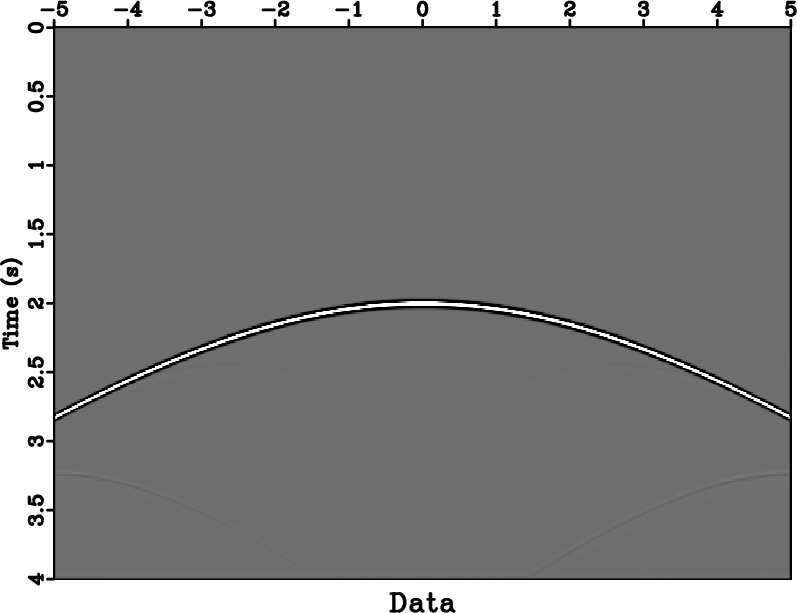
\includegraphics[scale=0.3]{/home/vgolubev/work/github/acinverse/madagascar/report/Fig/Figure_1.png}
  \caption{Сейсмограмма с одной прямой границей.}
\label{seismo_1}
\end{figure}

Также имеется возможность построения Zero-Offset сейсмограммы, т.е. когда каждая сейсмотрасса получена в условиях совпадения координат источника и приёмника.
На рисунке \ref{seismo_2} показана ZO-сейсмограмма для той же самой модели среды.
Использовался 2001 источник-приёмник с интервалом 50 м на всё протяжении расчётной области.

\begin{figure}[ht]
  \center
  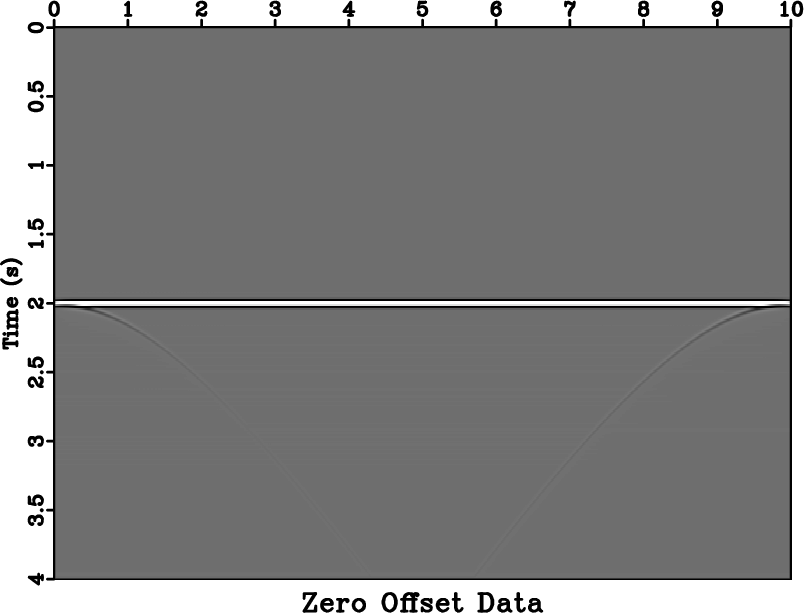
\includegraphics[scale=0.3]{/home/vgolubev/work/github/acinverse/madagascar/report/Fig/Figure_2.png}
  \caption{ZO-cейсмограмма с одной прямой границей.}
\label{seismo_2}
\end{figure}

При этом программа kirmod позволяет получить синтетическую сейсмограмму для произвольного распределения отражающих границ в пространстве.
Например, их можно задавать аналитическими функциями.
Для примера была рассчитана модель среды с тремя отражающими горизонтами, два из которых криволинейные.
Границы задавались функциями $(3.0 - 0.1 * x_1$, $0.5 * exp((x_1 - 5.0)^2 / 25) - 0.4$ и $-3.0 + 0.1 * x_1 + exp((x_1 - 5.0)^2 / 25) - 0.8$ соответственно.
Параметры расстановки выбирались аналогично предыдущему расчёту.

\begin{figure}[ht]
  \center
  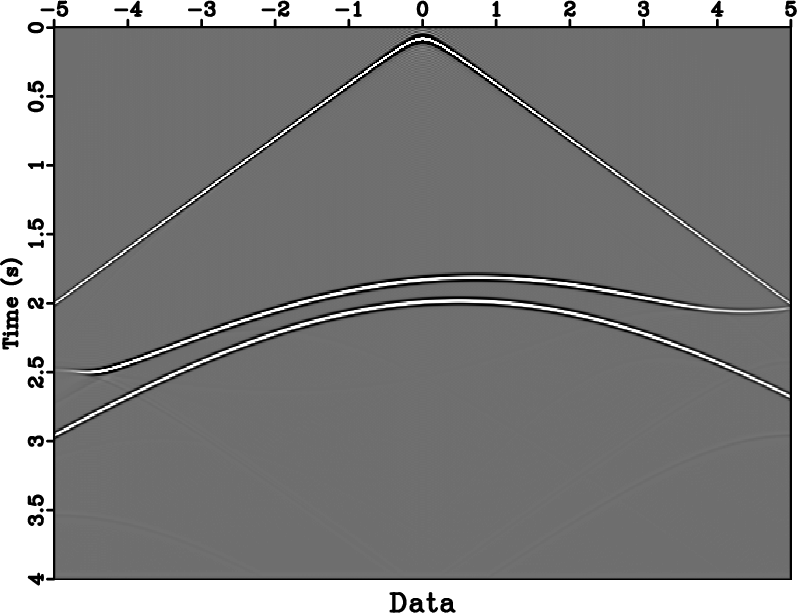
\includegraphics[scale=0.3]{/home/vgolubev/work/github/acinverse/madagascar/report/Fig/Figure_3.png}
  \caption{Сейсмограмма для модели с тремя отражающими горизонтами.}
\label{seismo_3}
\end{figure}

\begin{figure}[ht]
  \center
  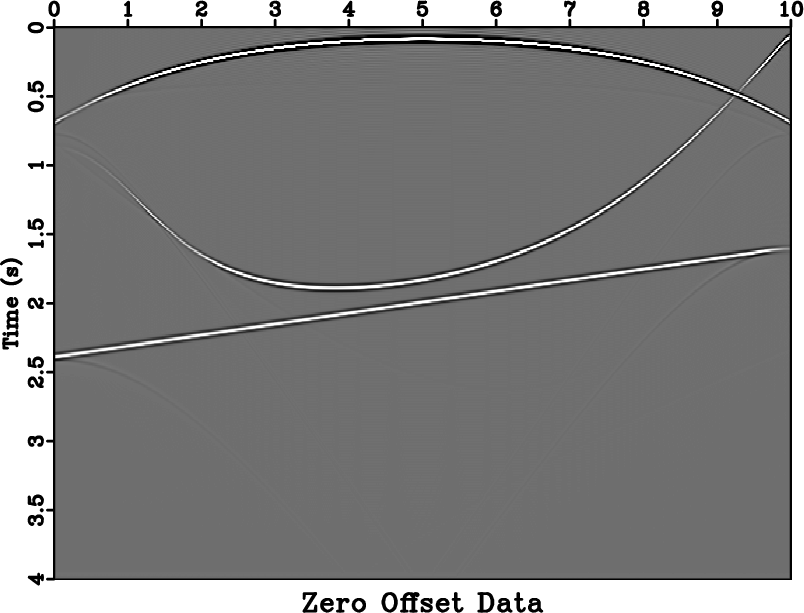
\includegraphics[scale=0.3]{/home/vgolubev/work/github/acinverse/madagascar/report/Fig/Figure_4.png}
  \caption{ZO-сейсмограмма для модели с тремя отражающими горизонтами.}
\label{seismo_4}
\end{figure}

\fi

\section{Сравнительный анализ двух алгоритмов на простых моделях}

Одной из целей работы являлось сравнение двух методов миграции (Кирхгоф и присоединённый оператор), реализованных в программах AcInverse и Borni.
Исследовалась 2D модель с двумя отражающими горизонтами\footnote{При расчёте сейсмограммы в Borni отражающие границы образовывались как результат включения одной большой неоднородности с $\delta s = 4*10^{-6}$}, которые задавались формулами:
\begin{itemize}
\item $z=-2$,
\item $z=-2 + (0.1 * x + 0.5)$.
\end{itemize}
Фоновая скорость распространения продольных волн 2500 м/с, геометрия расчётной области 10 км x 5 км.
Временная функция источника - Риккер с основной частотой 25 Гц.
В измерительную систему входил 201 источник и 201 приёмник, установленные каждые 50 м.

На рисунке \ref{seismo_verif_zo_madagascar_borni} (слева) приведена Zero-Offset-сейсмограмма, рассчитанная методом Кирхгофа (Madagascar, kirmod), а справа - программой Borni.
Как видно, Кирхгоф дал более чёткое изображение, хотя и с наличием сферических артефактов у границ области.
Таким образом, для тестирования алгоритмов миграции было получено два набора входных данных разными методами.

\begin{figure}[ht]\center
\begin{tabular}{cc}
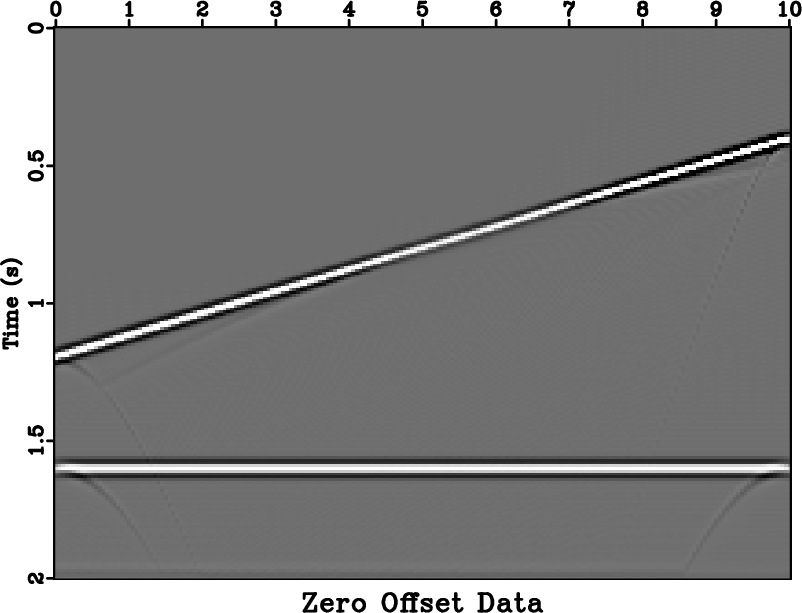
\includegraphics[width=50mm]{/home/vgolubev/work/github/acinverse/madagascar/report/Fig/seismo_verif_zo_madagascar_borni-madagascar.png}
&
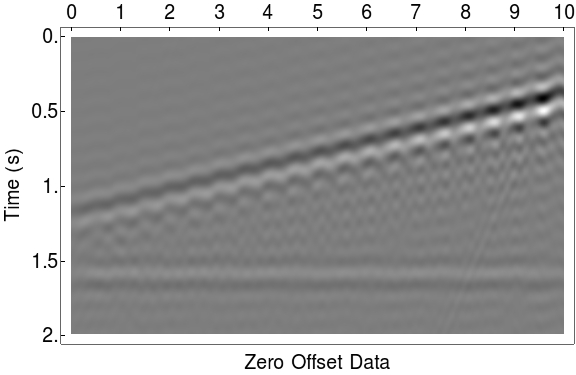
\includegraphics[width=60mm]{/home/vgolubev/work/github/acinverse/borni/seismo_verif_zo_madagascar_borni-borni.png}
\end{tabular}
\caption{ZO-сейсмограмма для верификационной модели. Слева - Madagascar, справа - Borni.}
\label{seismo_verif_zo_madagascar_borni}
\end{figure}

На рисунке \ref{seismo_verif_madagascar_borni-acinverse} представлены миграционные изображения, полученные методом Кирхгофа (AcInverse).
Можно говорить о выделяемости контактных границ, пусть и с небольшим контрастом и наличием артефактов.

\begin{figure}[ht]\center
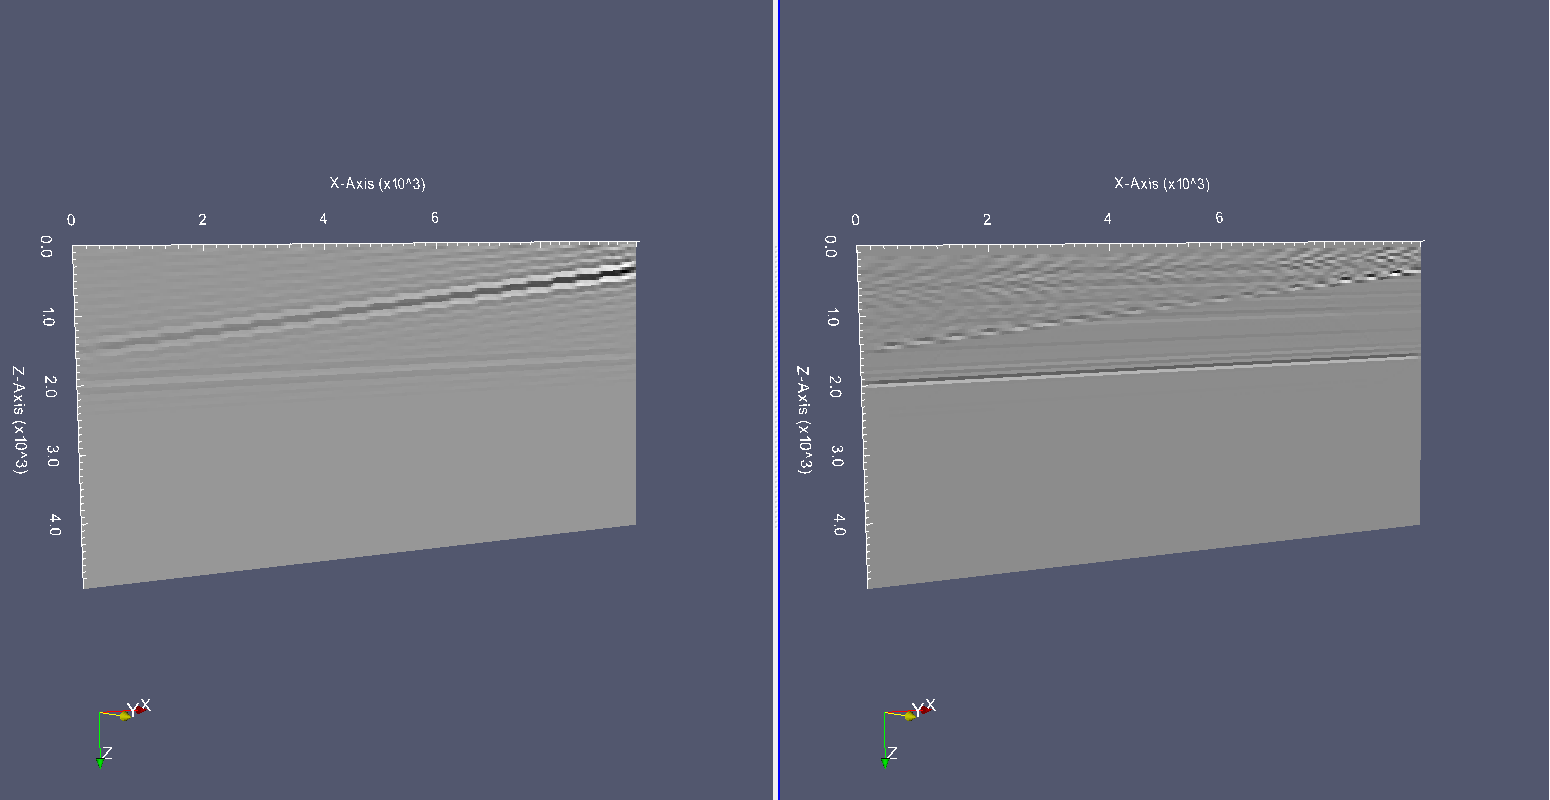
\includegraphics[width=100mm]{/home/vgolubev/work/github/acinverse/madagascar/report/Fig/seismo_verif_madagascar_borni-acinverse.png}
\caption{Миграционное изображение для верификационной модели, полученное методом Кирхгофа (AcInverse). Слева - на входе Борн (Borni), справа - на входе Кирхгоф (Madagascar).}
\label{seismo_verif_madagascar_borni-acinverse}
\end{figure}

На рисунке \ref{seismo_verif_madagascar_borni-borni} представлены миграционные изображения, полученные методом присоединённого оператора (Борн, Borni).

\section{Направление дальнейшего исследования}

В мартовский отчёт планируется включить приведённое выше сравнение методов миграции на трёхслойной модели в рамках задачи "Сравнительный анализ двух алгоритмов на простых моделях" и отдельные исследования (теория, чувствительность к параметрам) процедур миграции по Кирхгофу и Adjoint operator (Borne approximation).

Кроме того сформулированы направления дальнейшего исследования, с приоритетом которых нет чёткой определённости: 

\begin{enumerate}
\item Провести детальное исследование поведения алгоритмов миграции (AcInverse, Borni) при изменении расчётных параметров.
\item Провести верификационные сравнения таким же способом (К-К, Б-Б, К-Б, Б-К) на 2Д слоистых моделях с криволинейными границами, т.о. усложнив "простые модели".
\item Освоить в Madagascar решение прямой задачи FD методом (или доработать сеточно-характеристический метод), получить синтетическую ZO-сейсмограмму от верификационной трёхслойной модели и попробовать применить миграцию AcInverse и Borni.
\item Продлить границы 2Д модели вдоль третьей оси, чтобы получить 3Д, и провести верификационное тестирование на полученной 3Д модели.
\item Освоить Madagascar с целью построения ZO-сейсмограммы для сложной модели (например, Marmousi) и попробовать применить миграцию AcInverse и Borni.
\item Доработать Borni для реализации regularized least-square migration.
\item Перейти к построению матрицы L на основе finite-difference approximation, а потом реализовать аналог Borni на её основе.
\end{enumerate}

\begin{figure}[ht]\center
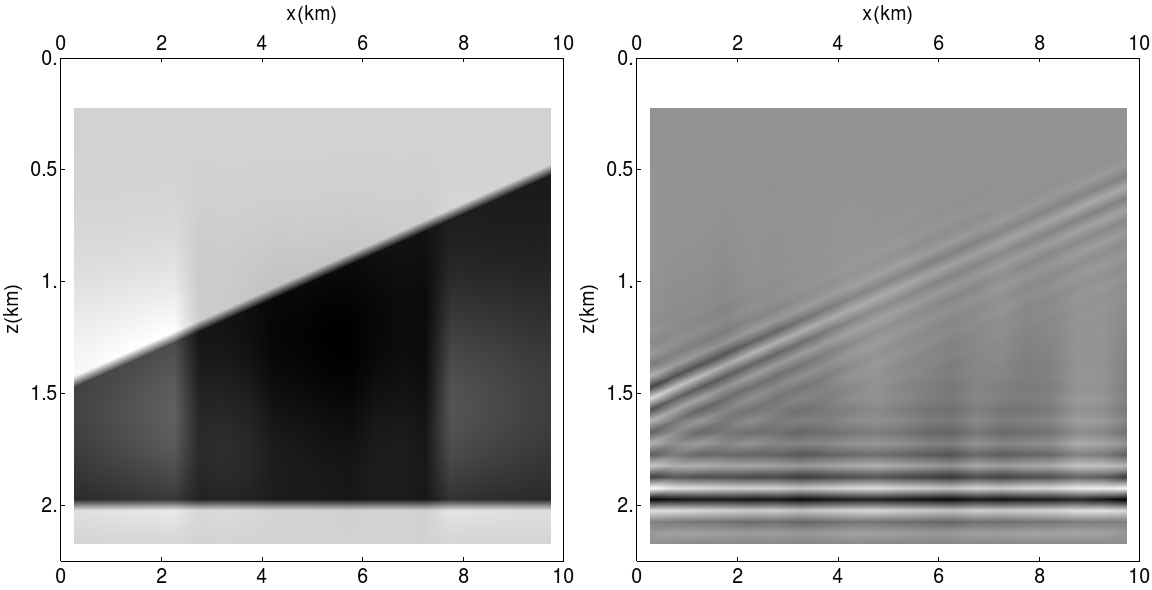
\includegraphics[width=120mm]{/home/vgolubev/work/github/acinverse/borni/seismo_verif_madagascar_borni-borni.png}
\caption{Миграционное изображение для верификационной модели, полученное методом присоединённого оператора (Борн, Borni). Слева - на входе Борн (Borni), справа - на входе Кирхгоф (Madagascar).}
\label{seismo_verif_madagascar_borni-borni}
\end{figure}

\if 0

\section{Заключение}

\section{Список литературы}
1. R.A.W. Haddon and P.W. Buchen "Use of Kirchhoff's formula for body wave calculations in the Earth" // Geophys. J.R. astr. Soc. (1981) 67, 587-598.

\fi

\end{document}
